\chapter{MULTILAYER DRIPPING HANDRAL}
    \label{chap:multilayer_dripping_handrail}
    \thispagestyle{empty}
    \mquote{Essentially, all models are wrong, but some are useful.}{George E. P. Box}

    As discussed in Chapter \ref{chap:similary_of_nonlinear_systems}, some models of physical systems can be very computationally demanding, so a simpler and manageable model analogy is often needed. For example, if we wanted to simulate the accretion disk system without simplification, it would be almost impossible to compute in the authors' lifetime. Such a model would be composed of individual and interacting gas particles. It would require either plasma physics equations or Navier-Stokes equations with a magnetic field; at that point, it is not a model but a perfect analogy. 

    The model developed for this study provides a manageable and reasonably complex tool for accretion disk simulation. Based upon its apparent characteristics, we call it \emph{Multilayer Dripping Handrail} (MDH) because it is an arrangement of concentric rings (i.e., layers). Each layer consists of up to several hundred cells, and each behaves as a \emph{dripping faucet}. The dripping mechanism drives the distribution of matter through the layers until they reach the central object.

% ---------
% The Model
% ---------
\section{The model}
    The MDH model is inspired by the model created by \citep{yonehara1997}. However, our model takes this concept much further. Instead of a simple mass limit condition, we use a slightly modified implementation of the Mass-Spring model (MSM) as a means of non-linear matter redistribution. We discussed the original MSM in detail in Chapter \ref{chap:dripping_faucet}. 

\subsection{The cellular accretion disk model}
    The concept of cellular automaton (CA) is quite an old idea in computer science that Stanislaw Ulam and John von Neuman first discovered at Los Alamos National Laboratory. However, it gained wider popularity after the publishing of \emph{Conway's Game of Life} \citep{gardner1970} and also extensive studies done by Stephen Wolfram starting in the 1980s.

    CA definition provided by \citep{wolfram2002} states that: \emph{Cellular automaton is a collection of cells on a grid of specified shape that evolves through a number of discrete time steps according to a predefined set of rules based on neighboring cells.} In our case, this set of rules mainly deals with distributing matter between the cells and throughout the accretion disk body.

    MDH is a cellular automaton that arranges $I$ times $J$ cells in a concentric ring (i.e., layers) grid pattern. The layers a denoted by 

    \begin{equation}
        i \in [0;I-1].
    \end{equation}

    The layer $i=0$ represents the outer edge layer of the disk. Each layer contains $J$ individual cells denoted by

    \begin{equation}
        j \in [0;J-1].
    \end{equation}

    Because the orbital angular velocities of individual layers differ, the simulation grid naturally shifts over time. Figure \ref{fig:grid_states} demonstrates the possible simulation grid states. On the left, we see the non-shifted initial state of the simulation. On the right, the layers of cells are slightly shifted after an arbitrary number of simulation steps.

    \begin{figure}[H]
    \centering
    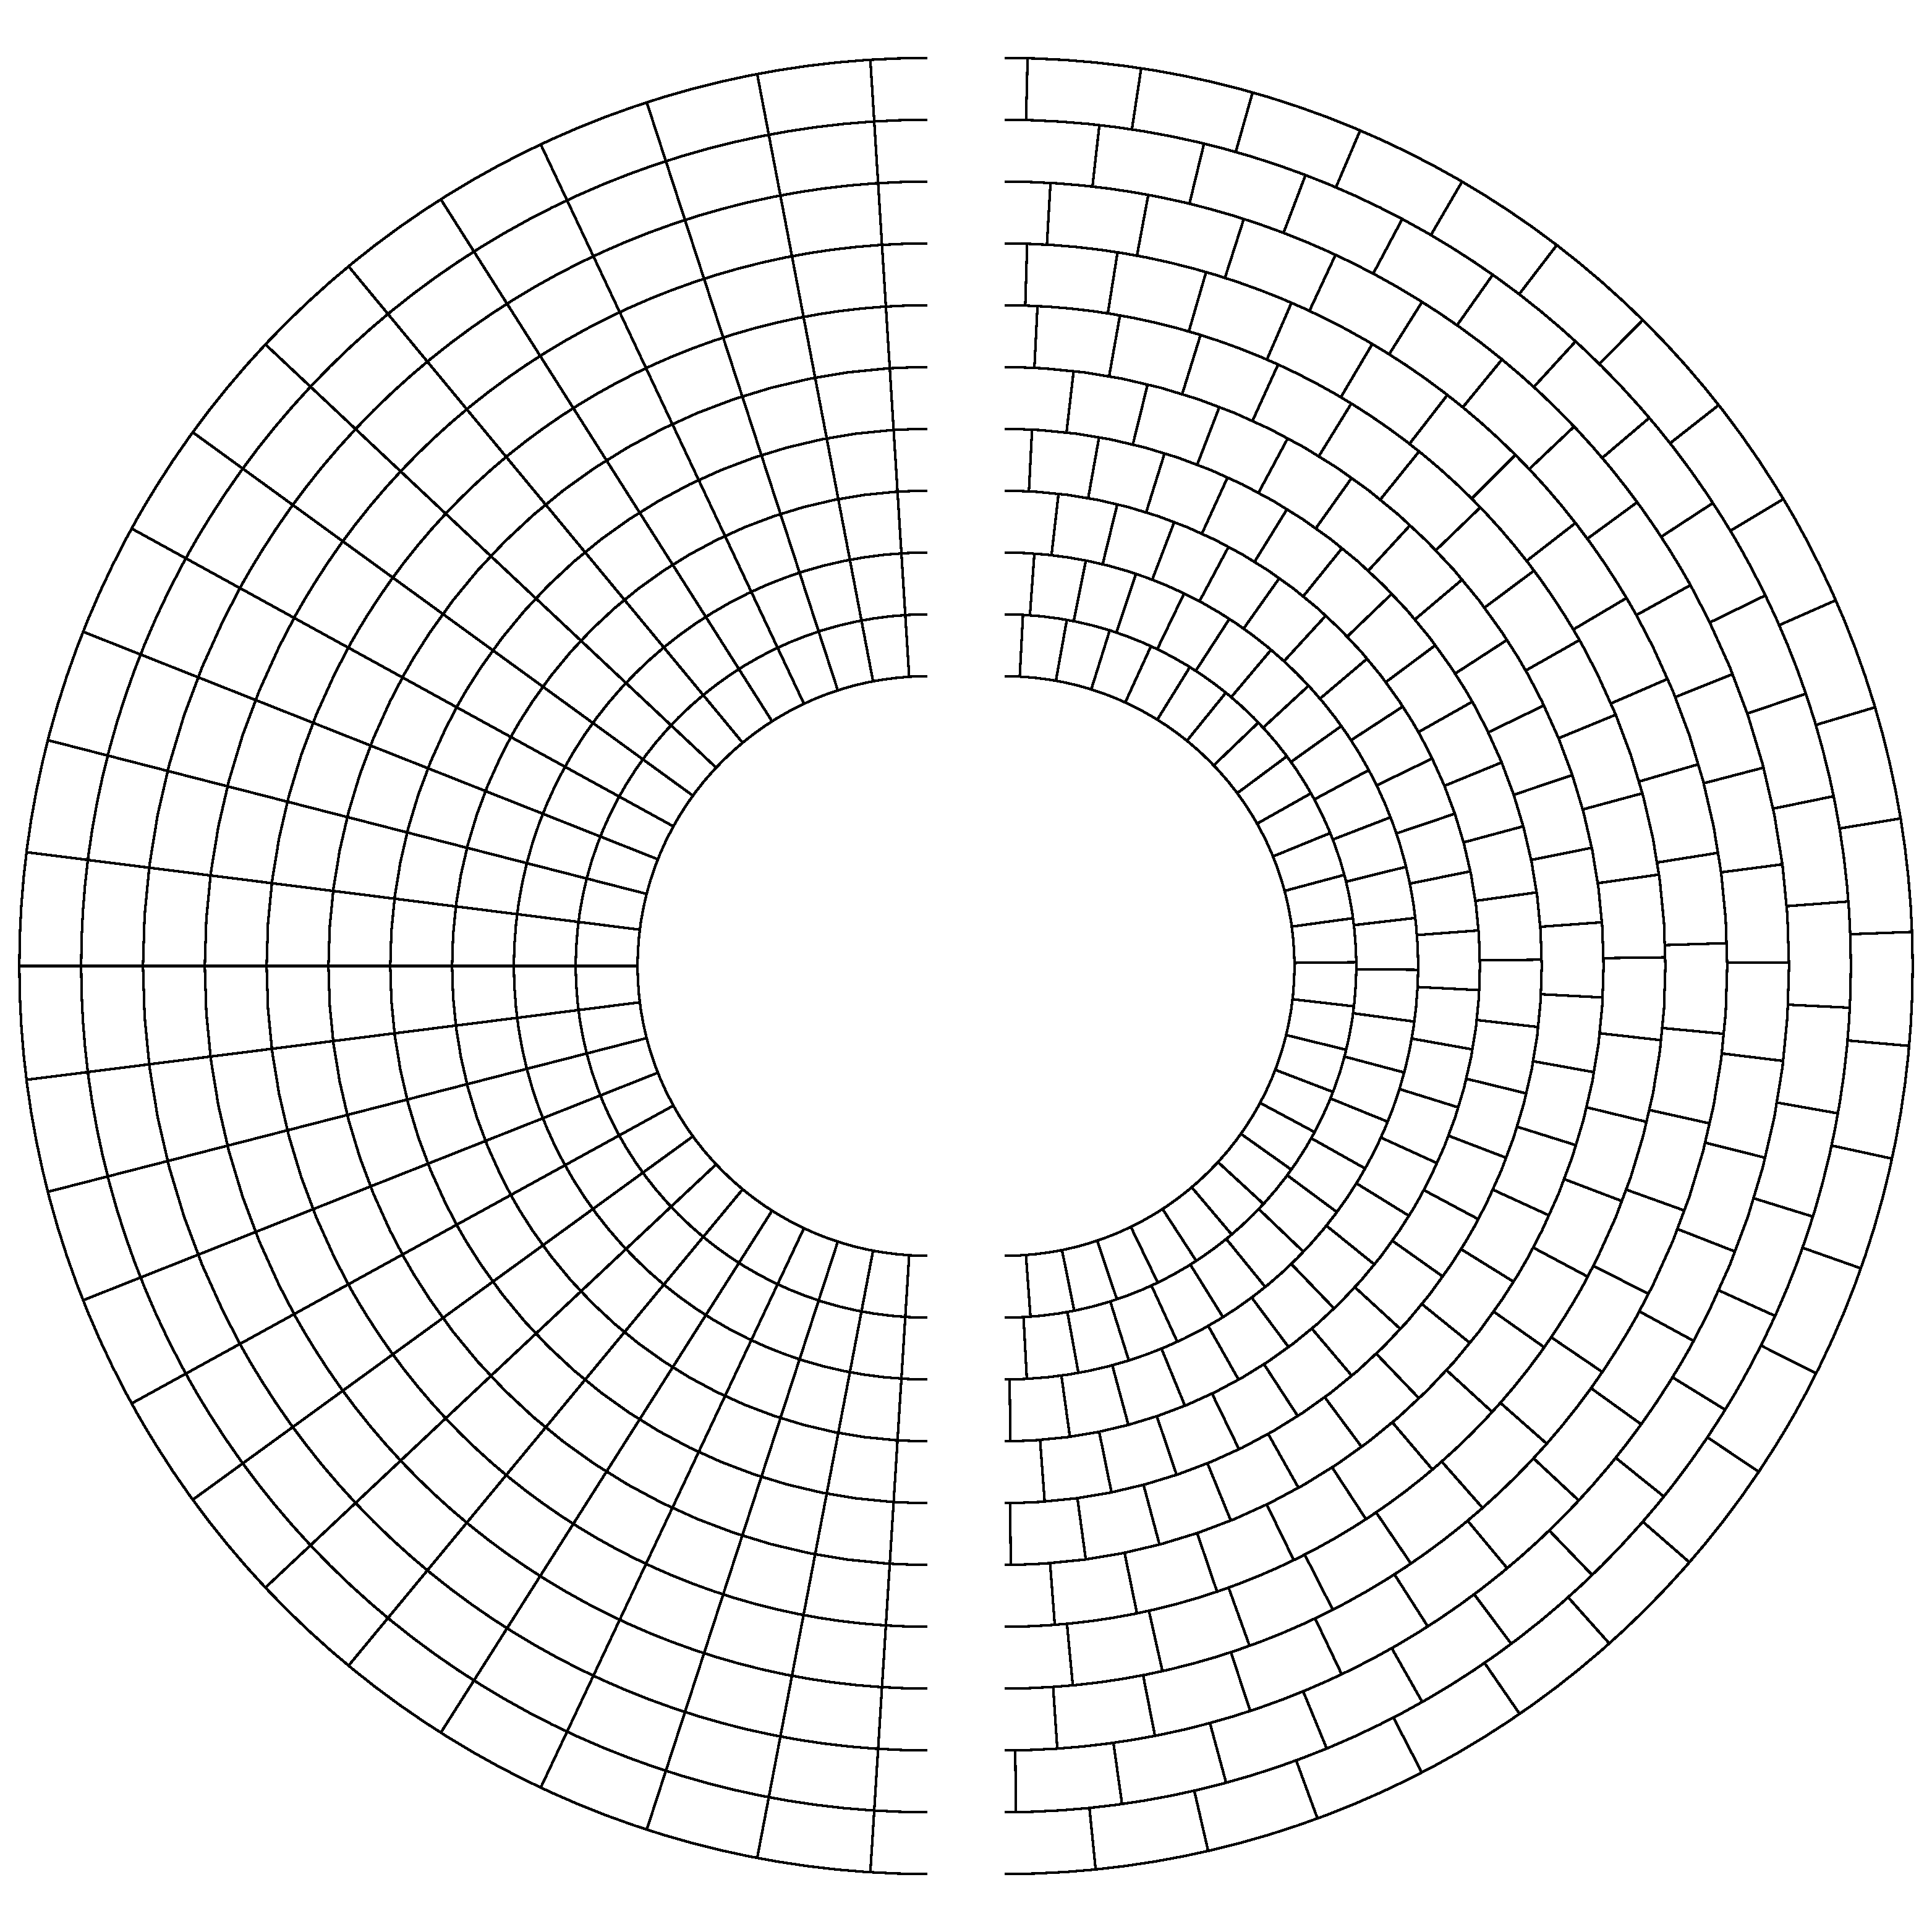
\includegraphics[width=\columnwidth]{img/grid_states.pdf}
    \caption{Grid states. Initial grid state (left) and shifted state after some arbitrary number of simulation steps (right).}
    \label{fig:grid_states}
    \end{figure}

    In the original MSM defined by \eqref{eq:msm_original_odes}, gravitational acceleration is a constant value. In our modification, it is substituted by $f_g$. We call this layer-dependent function the \emph{gravity profile} 

    \begin{equation}
        f_{\mathrm{g}}(i) = \frac{g_i}{g_{\mathrm{out}}},
        \label{eq:gravity_profile_0}
    \end{equation}

    where $g_{\mathrm{out}}$ represents the gravitational acceleration in the outer layer $i=0$, and $g_i$ in $i$th layer, and its value is ${f_{\mathrm:TagbarToggle
    {g}}(i=0) = 1}$ (same as the original MSM). In any layer, the $g_i$ value is 

    \begin{equation}
        g_i = \frac{GM_{\mathrm{p}}}{r_i^2},
        \label{eq:gravity_profile_layer}
    \end{equation}

    where $G$ is the universal gravitational constant, and $M_{\mathrm{p}}$ is the mass of the primary component (i.e., the white dwarf). We substitute \eqref{eq:gravity_profile_layer} into \eqref{eq:gravity_profile_0} the $GM_{\mathrm{p}}$ components cancels out, and the resulting \emph{gravity profile} function depends only on layer index $i$

    \begin{equation}
        f_{\mathrm{g}}(i) = \left( \frac{r_{\mathrm{out}}}{r_i} \right)^2.
        \label{eq:gravity_profile_final}
    \end{equation}


    Because the orbits are considered Keplerian, angular velocities also differ between layers. Therefore, a function similar to \emph{gravity profile} is needed to correctly handle the rotation of individual layers throughout the simulation. The assumption is that if the outer layer moves by one angular cell length in one step, then any subsequent layer moves by some more. This function $f_{\omega}$ is referred to as \emph{angular velocity profile}

    \begin{equation}
        f_{\omega}(i) = \frac{\omega_i}{\omega_\mathrm{out}},
        \label{eq:av_profile_0}
    \end{equation}

    where $\omega_{\mathrm{out}}$ is the outhermost layer's angular velocity and $\omega_i$ of an arbitrary layer, which is 

    \begin{equation}
        \omega_i = \frac{v_i}{r_i},
        \label{eq:omega_layer}
    \end{equation}

    where $v_i$ is the orbital velocity, which we get from the relation

    \begin{equation}
        v_i^2 = \frac{G M_{\mathrm{p}}}{r_i}.
        \label{eq:velocity_layer}
    \end{equation}

    Substitution of \eqref{eq:velocity_layer} into \eqref{eq:omega_layer} and than into \eqref{eq:av_profile_0} gives us the \emph{angular velocity profile} function

    \begin{equation}
        f_{\omega}(i) = \left(\frac{r_{\mathrm{out}}}{r_i}\right)^{3/2}.
    \end{equation}

    To get the change of cell's angular position $\theta$ (i.e., the azimuth) we apply the function $f_{\omega}(i)$ in conjuction with grid's dimension $J$

    \begin{equation}
        \Delta \theta (i) = f_{\omega} \frac{2 \pi}{J}.
        \label{eq:delta_azimuth} 
    \end{equation}

    The expression \eqref{eq:delta_azimuth} fully describes the angular shift of arbitrary cells in between simulation steps. Figure \ref{fig:plot_omega_g_profiles} shows examples of both aforementioned profiles.
    
    \begin{figure}[H]
    \centering
    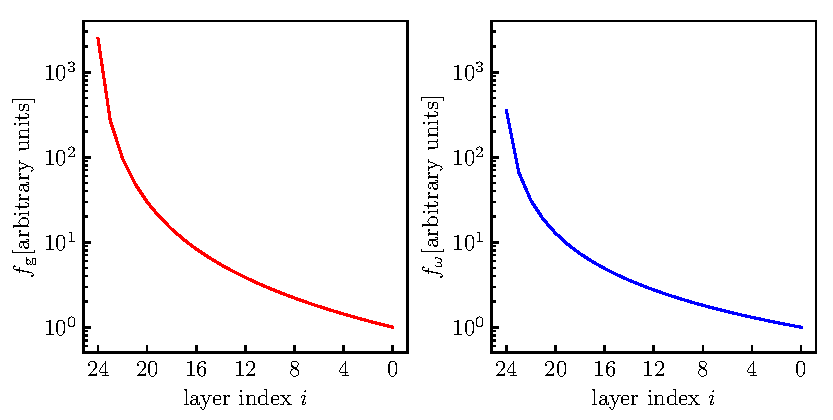
\includegraphics[width=\columnwidth]{img/plot_omega_g_profiles.pdf}
        \caption{Gravity (left) and angular velocity (right) profiles examples computed for a modeled system with radial dimension $I = 25$. The y-axis units are arbitrary because the profiles are computed relative to the outermost layer $i = 0$, where $f_{\mathrm{g} = 1}$ and $f_{\omega} = 1$.}
    \label{fig:plot_omega_g_profiles}
    \end{figure}
        
    Lastly, in our modification, $Q$ depends on the specific behavior of neighboring cells, unlike the original value defined by \eqref{eq:ode_2}. Each cell essentially contains its \emph{leaky faucet}, taking the mass from other cells and redistributing it further into lower cells upon reaching the critical condition. This critical condition $z_{\mathrm{c}}$ is the same as the original MSM and is defined by \eqref{eq:z_critical_model}.

    To summarize our modification to the original MSM, the following modified ODE system server a mechanism by which the matter redistribution is triggered inside simulation cells of the MDH model

    \begin{align}
    \begin{split}
        \D{}{t} \left(m \D{z}{t}\right) &= -kz - \gamma\D{z}{t} + m f_{\mathrm{g}}, \\
        \D{m}{t} &= Q(i, j, ...),
    \end{split}
    \label{eq:msm_modified_odes}
    \end{align}

\subsection{Modeled system geometry and grid dimensions}
    Our primary focus is modeling an accretion disk of a typical \emph{cataclysmic variable star}, where the primary component would be a WD. Mass of the WD $M_{\mathrm{p}}$ can range from $0.15 M_{\odot}$ up to $1.44 M_{\odot}$, and the heaviest observed white dwarf has a mass of $1.35 M_{\odot}$ \citep{caiazzo2021}, therefore we are limited to this range when choosing primary component's mass $M_{\mathrm{p}}$.

    The inner disk radius $r_{\mathrm{in}}$ is set equal to the white dwarf's radius, which according to \citep{shapiro1983}, can be approximated by the \emph{mass to radius ratio} previously defined by \eqref{eq:mass_radius_ratio}.

    The Roche lobe of the primary component contains the outer edge of the accretion disk. Therefore the outer radius $r_{\mathrm{out}}$ is set to correspond with the binary system's Lagrange point $L_1$ and is calculated by \eqref{eq:disk_outher_radius}. Mass of the donor component $M_{\mathrm{s}}$, which also plays a role in determining the accretion disk's outer radius through its influence on Roche potential, ranges between $0.3M_{\odot}$ and $8M_{\odot}$ because the secondary star is considered to be a red-giant. 

    Having the inner and outer disk boundaries defined enables the discretization of the intermediate space into regular intervals, and the remaining parameter influencing the layer-specific radius $r_i$ is the disk's dimension $I$

    \begin{equation}
        r_i = r_{\mathrm{in}} + \frac{r_{\mathrm{out}} - r_{\mathrm{in}}}{I - 1} (I - i - 1).
    \end{equation}

    On a Keplerian orbit, the particle's orbital period, assuming there is no self-gravity interaction in the disk, is given only by the parameters $M_{\mathrm{p}}$ and $r_i$. 


    We also assume that the outermost layer of MDH shifts by exactly one \emph{angular cell length} between simulation steps. Therefore the $J$ dimension (i.e., the number of cells in one layer) and primary component's parameters provide us with the shortest producible flickering time.

    We aim to extract flickering light curves with a time scale of variability comparable to real-world observational data. Observations suggest that we need to push this time limit $\Delta t$ at least to the order minutes. To get relate the dimension $J$ and the minimal time $\Delta t$, the orbital period $\tau_{0}$ for the layer $i=0$ is needed

    \begin{equation}
        \tau_{0} = \sqrt{\frac{4 \pi^2 r_{\mathrm{out}}^3}{G M_{\mathrm{p}}}},
        \label{eq:outer_layer_tau}
    \end{equation}

    where $G$ represents the gravitational constant. So the optimal $J$ dimension is calculated

    \begin{equation}
        J = \frac{\tau_{0}}{\Delta t}.
        \label{eq:j_dimension}
    \end{equation}

    Rounding the result of \eqref{eq:j_dimension} to integer gets us the $J$ dimension for chosen minimal time $\Delta t$. Alternatively, there is a possibility of using the expression \eqref{eq:j_dimension} in reverse, starting with the chosen dimension, and the relation will give the time scale for the particular arrangement.

    The $I$ dimension is either set to a fixed chosen value or is related to the $J$ dimension. Choosing a relation that produces, at least to some degree, a spatially consistent grid of cells is advised. Throughout this study, we use the following relation, which is, again, rounded to an integer 

    \begin{equation}
        I = \frac{J}{2 \pi}.
        \label{eq:i_dimension} 
    \end{equation}

\subsection{The cellular automaton algorithm}
    The algorithm that performs the MDH simulations is a series of simple operations, including matter redistribution (i.e., the \emph{dripping} mechanism), orbital movement of its layers, and thermal processes, which are the prerequisite for light curves extraction. The algorithmic structure overview of MDH simulation is defined on the flowchart shown in figure \ref{fig:diagram_cellular_algorithm}. 

    Certain parts of the algorithm are relatively easy to parallelize, most notably the numerical solution of the ODE system \eqref{eq:msm_modified_odes}. Parallelization is almost a necessity because the number of cells for which we need to solve these equations quickly goes to thousands, even when using modest $I$ and $J$ dimensions of tens or a few hundreds of cells per dimension. Thankfully the MSM equations in individual cells are not dependent on other cells' states, so splitting the grid of solutions into multiple smaller sub-grids of tasks per step is relatively straightforward.

    \vspace*{2mm}
    
    \begin{figure}[H]
    \centering
    \begin{tikzpicture} [node distance=2cm]
        \node (start) [startstop] {Start}; 
        \node (pr1) [process, below of=start, yshift=-0.5cm] {Rotate all layers according to \eqref{eq:delta_azimuth}.}; 
        \node (pr2) [process, below of=pr1, yshift=-1cm, inner sep=0.25cm] {Find the cell closest to chosen value of $\theta$ (e.g., $\theta = 0$) in the outer layer $i = 0$, and add the $q$ amount of matter to it; see \eqref{eq:q_estimate}.}; 
        \node (pr3) [process, below of=pr2, yshift=-1.5cm] {Solve the ODE system \eqref{eq:msm_modified_odes} for all cells using an iterative method out of the Runge-Kutta family.}; 
        % TODO: pridat referenci na popis RK metod v kapitole o implementaci
        \node (if1) [decision, below of=pr3, yshift=-1cm] {If particular cell reaches the critical condition \eqref{eq:z_critical_model}, the mass outflow is triggered in that cell.}; 
        \node (pr4) [process, right of=if1, xshift=5.5cm] {Calculate temperature changes for all cells according to the processes described in Section \ref{sec:thermal_processes}};
        \node (pr6) [process, right of=pr2, xshift=5.5cm] {Save all cell's states.};
        \node (if2) [decision, right of=pr1, xshift=5.5cm] {End simulation?};
        \node (pr5) [process, below of=if1, yshift=-1.0cm] {Perform mass outflow of triggered cells; see \eqref{eq:delta_m}.};
        \node (stop) [startstop, right of=start, xshift=5.5cm] {Stop};

        \draw[arrow] (start) -- (pr1);
        \draw[arrow] (pr1) -- (pr2);
        \draw[arrow] (pr2) -- (pr3);
        \draw[arrow] (pr3) -- (if1);
        \draw[arrow] (if1) -- node[anchor=east] {yes} (pr5);
        \draw[arrow] (if1) -- node[anchor=south] {no} (pr4);
        \draw[arrow] (pr5) -| (pr4);
        \draw[arrow] (pr4) -- (pr6);
        \draw[arrow] (pr6) -- (if2);
        \draw[arrow] (if2) -- node[anchor=south] {no} (pr1);
        \draw[arrow] (if2) -- node[anchor=east] {yes} (stop);
    \end{tikzpicture}
        \vspace*{1mm}
    \caption{The algorithmic structure overview of MDH simulation. }
    \label{fig:diagram_cellular_algorithm}
    \end{figure}

    The discrepancy needed to be dealt with when simulation MDH is that MSM's mass scale is different from the global (i.e., real-world) mass scale of the accretion disk. However, it is not a big problem. MSM is used only as the critical condition because of its qualitative and not quantitative properties. Nevertheless, we need to know the \emph{real} amount of accreted matter. For a typical CV, the accretion rate is assumed \citep{ae_shortrev2015}

    \begin{equation}
        \dot{M} \sim 10^{14}\, \mathrm{g \cdot s^{-1}},
    \end{equation}

    and the value of $a$ according to \citep{msmm1999} is

    \begin{equation}
        \label{eq:q_estimate}
        q \sim 10^{-1}\, \mathrm{g},
    \end{equation} 

    so, we can easilly relate the \emph{real} accretion rate $\dot{M}$ to the internaly defined $q$

    \begin{equation}
        q \propto \dot{M} \cdot \Delta t.
    \end{equation}

    The mass addition to the outer layer $i = 0$ that models the matter accretion through the Lagrange point $L_1$ would fill up only the outer layer. Therefore the subsequent layers are filled from the adjacent cells \emph{above} when they reach the critical condition \eqref{eq:z_critical_model}.

    Part of the mass is separated from the source cell as the moment of \emph{dripping} and transfers into lower cells. The amount of mass $\Delta m$ that breaks is

    \begin{equation}
        \Delta m = \psi \cdot m_{ij}
        \label{eq:delta_m}
    \end{equation}

    where the value of $\psi \in [0;1]$ is the drop breakout ratio, which serves as another free parameter of the simulation. The numerical stability of the simulation is ensured by introducing a low-value cut-off for the cell's mass $m_{ij}$. The following formula is used to compute the cell's remaining mass after the breakout    
    % TODO: zahrnout psi mezi volne parametry v pozdejsich vypoctech!!

    \begin{equation}
        \begin{aligned}
            & m_{ij}~= 
            \begin{cases}
                m_{ij} - \Delta m \hspace{5mm} (m_{ij} \ge 10^{-8}) \\
                \hspace{8mm} 0 \hspace{12.5mm} (m_{ij} < 10^{-8}).
            \end{cases}
        \end{aligned}
        \label{eq:m_cut_off}
    \end{equation}

    There are always no more than two lower layer cells in contact with the source cell, as evident from Figure \ref{fig:grid_states}. Therefore, the redistribution algorithm finds the two closest cells and splits the mass $\Delta m$ between the two receiving cells. The mass split is directly proportional to the relative length of contact the adjacent cells have with the source cell.

% -----------------
% Thermal processes  
% -----------------
\section{Thermal processes}
\label{sec:thermal_processes}
    The crucial quantity for our model's evaluation is the extracted synthetic light curve, which we derive from the disk's radiation properties, primarily the temperature. The temperature must be known for all cells at any moment of the simulation. We assume that the cells exhibit black-body radiation and are optically thin. 

    The cell temperature continuously changes and depends on the previous states rather than being a function of only current internal and external parameters. Because of the matter redistribution processes (i.e., the dripping and rotational mixing), the temperature changes are carried throughout the disk's body. The starting point of this chain of changes is matter inflow in the outer layer $i = 0$. The given parameters of the donor star determine the inflow temperature. For the late-type star, according to \citep{allen1973}, it is estimated

    \begin{equation}
    T_{\mathrm{out}} \sim 10^3\, \mathrm{K}.
    \end{equation}

    We identified three processes influencing the cell's temperature. In the following sections, we will describe those in detail and get the final cell's temperature as their summary. 

\subsection{Free-Free emission heating}
    The matter that beaks out by \emph{dripping} losses a part of its potential energy, which, according to \citep{yonehara1997}, is calculated by 

    \begin{equation}
    \Delta E_{ij} = \frac{1}{2} G M_{\mathrm{p}} \Delta r \frac{\Delta m_{ij}}{r_i^2},
    \label{eq:e_pot}
    \end{equation}

    where the amount of falling mass is represented by $\Delta m_{ij}$ and $\Delta r$ is the layer width (i.e., the distance traveled by the mass). This energy is released by the process of \emph{free-free emission} (i.e. bremsstrahlung); with some efficiency $\varepsilon$ is transformed into internal energy $U$ of the receiving cell

    \begin{equation}
        \Delta U_{i+1,j} = \varepsilon \Delta E_{ij},
    \end{equation}

    where $\Delta U_{i+1,j}$ represents the change of receiving cell's internal energy that heats the cell. For the sake of simplicity, we consider the heating efficiency to be ${\varepsilon=1}$, then  

    \begin{equation}
        \Delta U_{i+1,j} \equiv \Delta E_{ij}.
        \label{eq:e_int_pot_equiv}
    \end{equation} 

    Internal energy changes in relation to the temperature according to 

    \begin{equation}
        \Delta U_{ij} = \frac{3}{2} n_{ij} \mathcal{R} \Delta T_{ij},
        \label{eq:e_int_temp_relation}
    \end{equation}

    where $\mathcal{R}$ represents the ideal gas constant, and $n_{ij}$ is the number of gas moles in the cell. We assume the gas mostly consists of hydrogen, whose molar mass is $M_{\mathrm{H}} \approx 1$; therefore, the mass $m_{ij}$ and the number of moles $n_{ij}$ are interchangeable. Substitution of \eqref{eq:e_int_temp_relation} and \eqref{eq:e_pot} into \eqref{eq:e_int_pot_equiv}, and a bit of rearrangement, yields the relation of cell's temperature change in layer $i+1$, and the amount of mass falling from the donor cell

    \begin{equation}
        \Delta T_{i+1,j} = \frac{1}{3} \frac{G M_{\mathrm{p}} \Delta m_{ij} \Delta r}{r_{i}^2 \mathcal{R} m_{i+1,j}}.
        \label{eq:temp_ff_final}
    \end{equation}

\subsection{Gas mixing}
    The second mechanism concerns mixing different temperatures and amounts of gases when dripping happens. We need to describe the donor cell's temperature change $T_{ij}$ and the receiving cell's $T_{i+1,j}$. We get both by utilizing changes in the cell's internal energy. The resulting expression for the donor cells is simply  

    \begin{equation}
    T_{ij}' = T_{ij},
    \end{equation}

    where $T_{ij}$ and $T_{ij}'$ are the temperatures before and after the mass outflow, respectively. The mixing of two different amounts of gas at two different temperatures is happening on the receiving cell's side. The expression for the receiving cell is

    \begin{equation}
    T_{i+1,j}' = \frac{m_{i+1,j} T_{i+1,j} + \Delta m_{ij} T_{ij}}{m_{i+1,j} + \Delta m_{ij}}.
    \end{equation}

\subsection{Radiative cooling}
    The last mechanism taking part in the cell's temperature changes is radiative cooling. The cell's radiation of optically thin disk is approximated as black-body radiation that emits through the top and bottom facets of each cell, and one facet having the area

    \begin{equation}
        S_{ij} = \frac{2 \pi r_i \Delta r}{J},
        \label{eq:facet_area}
    \end{equation}

    where the layer width is represented by $\Delta r$. Therefore cell's internal energy conversion to its black-body radiation is

    \begin{equation}
        \frac{3}{2} m_{ij} \mathcal{R} \frac{dT_{ij}}{dt} = \sigma T_{ij}^4 S_{ij},
        \label{eq:rad_cooling_temp_0}
    \end{equation}

    where $\sigma$ is the Stefan-Boltzman constant. Integration of \eqref{eq:rad_cooling_temp_0} and yields the expression for the cell's temperature, which is in the local thermodynamic equilibrium of the radiative cooling

    \begin{equation}
    T_{ij}' = \left( \frac{2 \sigma S_{ij} t}{m_{ij} \mathcal{R}} + \frac{1}{T_{ij}^3} \right)^{-1/3}.
    \end{equation}

% --------------------------------
% Synthetic light curve extraction
% --------------------------------
\section{Synthetic light curves}
    Synthetic light curve extraction starts with the full knowledge of temperatures throughout the simulation as a product of previously defined thermal processes. This information enables us to extract simulated spectra from the disk's radiation. Wavelength-specific radiation power of individual cells is given by

    \begin{equation}
        L_{\lambda,ij} = 4\pi \cdot S_{ij} \cdot B_{\lambda,ij}(\lambda, T_{ij}),
        \label{eq:facet_radiation}
    \end{equation}

    where $B_{\lambda}(\lambda, T_{i,j})$ represents flux density in the given point by Planck's function. Single radiating facet area $S_{ij}$ is defined by \eqref{eq:facet_area}, and the accretion disk, considered optically thin, radiates through a single face into the solid angle of $2\pi$. 

\subsection{Light curves in a photometric filter}
    To achieve a closer observational data analogy, we use analytic approximations of Johnson-Cousins $\mathcal{UBVRI}$ filters that are applied to the wavelength-specific total power output of the disk. This filtering process produces the synthetic light curve as it would be observed through the chosen filter. The approximation is expressed by

    \begin{equation}
    g(\lambda) \propto \mathrm{exp}\left[ - \frac{1}{2} \left( \frac{\lambda - \lambda_{\mathrm{c}}}{\lambda_{\mathrm{w}}} \right)^2 \right],
    \label{eq:filter_gauss}
    \end{equation}

    where filter-specifig effective central wavelength is $\lambda_{\mathrm{c}}$, and $\lambda_{\mathrm{w}}$ sets the effective filter width. Johnson-Cousins approximative values are listed in Table \ref{tab:johnson_cousins_approx}.

    \begin{table}[ht]
    \centering
    \begin{tabular*}{\columnwidth}{@{\extracolsep{\fill}}ccc}
    Filter & $\lambda_{\mathrm{c}}$ $[\mathrm{\r{A}}]$ & $ \lambda_{\mathrm{w}}$ $[\mathrm{\r{A}}]$\\
    \hline\hline
    $\mathcal{U}$ & 3663 & 650\\
    $\mathcal{B}$ & 4361 & 890\\
    $\mathcal{V}$ & 5448 & 840\\
    $\mathcal{R}$ & 6407 & 1580\\
    $\mathcal{I}$ & 7980 & 1540\\
    \hline
    \end{tabular*}
    \caption{Parameters of Johnson-Cousins $\mathcal{UBVRI}$ filters approximation. \citep{bessell2005}}
    \label{tab:johnson_cousins_approx}
    \end{table}

    We calculate every cell's radiation power step by step. Using \eqref{eq:facet_radiation} and \eqref{eq:filter_gauss} and summing up all the cells, we get filtered power output $L_{\mathrm{F}}$ from both accretion disk's sides

    \begin{equation}
    L_{\mathrm{F}} = 4 \pi S_{ij} \Delta \lambda \sum_{i=0}^{I-1} \sum_{j=0}^{J-1} \sum_{\lambda=0}^{\infty} B_{\lambda,ij}(\lambda, T_{ij})\,g(\lambda),
    \end{equation}

    where $\Delta \lambda$ is the wavelength integration step.
